%\documentclass[11pt,a4paper]{report}
\documentclass[11pt,a4paper]{article}
%\documentclass[11pt,a4paper]{amsart}

\usepackage{listings}
\usepackage{amsmath}
\usepackage{verbatim}
\usepackage{graphicx}

\lstset{language=Python}

\title{Cylon: An Optimal Dynamic Metascheduler for Forecasting Systems}

\author{Hilary Oliver, NIWA}

\begin{document}

\maketitle

\pagebreak
\tableofcontents
\pagebreak

\begin{abstract}

    {\em Cylon} is a forecasting systems metascheduler\footnote{A {\em
    metascheduler} determines the order in which tasks are sent to the
    job scheduler(s), i.e.\ it decides when dependent tasks are {\em
    ready} to run. The term also describes a single aggregate view of
    multiple distributed resource managers, which is not the topic of
    this paper.} that abandons the system-wide forecast cycle in favour
    of explicit handling of intercycle dependencies between individual
    tasks.\footnote{A {\em task} is any group of processes treated as a
    single entity for scheduling purposes.} In a system controlled by
    cylon a series of distinct forecast cycles emerges naturally in real
    time operation, but in catch up operation, delayed parallel trials,
    or historical case studies, tasks from any number of forecast cycles
    can run simultaneously to the full extent allowed by dependencies,
    with the potential for greatly increased system throughput. Cylon is
    also extremely flexible and easy to use because each task simply
    registers its own inputs and outputs, as if to run alone, and
    dependencies are resolved at run time. The system thus adapts
    dynamically to insertion or removal of tasks at run time. Explicit
    handling of forecast model `restart' dependencies allows continued
    operation, with very little human intervention, over major failures
    that involve omitted forecast cycles in the driving models.  Control
    of the configured task set, and failure recovery scenarios, can be
    tested quickly in a simulation mode that is indistinguishable (to
    cylon) from real operation. Cylon is written in object oriented
    Python and uses the Python Remote Object Protocol ({\em Pyro}) to
    control tasks across a network. It is easily interfaced to existing
    tasks (models, post-processing, etc.).

\end{abstract}

\section{Forecasting Systems}
\label{sec:FS}

Environmental forecasting systems generate forecast products at regular
intervals from a set of linked scientific models and associated data
processing tasks. From a job scheduling perspective such a system
is a set of regularly repeating interdependent tasks, possibly with
different cycle periods, whose execution order must be carefully
controlled to avoid dependency violations. 

Normal real time operation necessarily consists of a series of distinct
{\em forecast cycles} that are initiated, after a gap in processing, by
new external driving data (typically real time observations and/or
forecast fields from an external system). Tasks are therefore naturally
grouped by {\em forecast cycle}, wherein each task has the same {\em
forecast reference time}, which is the nominal start time of the
forecast models in the cycle group, or that of the associated forecast
model run(s) for data processing tasks.

\subsection{EcoConnect}

The EcoConnect Forecasting System at the National Institute of Water and
Atmospheric Research (NIWA) in New Zealand takes real time atmospheric
and stream flow observations, and operational global weather forecasts
from the Met Office (UK), and uses these to drive global sea state and
regional data assimilating weather models, which in turn drive regional
sea state, storm surge, and catchment river models, plus tide
prediction, and a large number of associated data collection, quality
control, preprocessing, postprocessing, product generation, and
archiving tasks.\footnote{Plans for EcoConnect include additional
deterministic regional weather models and an weather model ensemble.}
The regional weather model runs four times daily in the 00, 06, 12, and
18 UTC cycles, but it supplies surface pressures to a regional storm
surge model that runs only twice daily, in the 00 and 12 UTC cycles, and
precipitation accumulations to catchment river models that run on an
hourly cycle as they assimilate real time stream flow observations.
EcoConnect runs on heterogenous distributed hardware, including a
massively parallel supercomputer and several Linux servers. 

\section{Task Dependencies}

One normally thinks of these dependencies as operating within a forecast
cycle. A sea state forecast, for example, might depend on surface wind
fields generated by an upstream weather forecast over the same forecast
range, and a product generation task can't run before its associated
forecast is finished. There are also dependencies between tasks in
different forecast cycles though: model forecasts typically depend on a
recent previous forecast (by the same model) for their initial
``background state'', and different kinds of tasks in different forecast
cycles can also be linked (c.f.\ the way in which the TopNet catchment
model depends on the weather model in EcoConnect). 

In real time operation, however, intercycle dependencies can be treated
as implicitly satisfied because one cycle necessarily finishes before
the next begins. Which is just as well because intercyle dependencies
dramatically increase apparent complexity of even the simplest systems,
by destroying the clean boundary between forecast cycles.

All existing forecasting control systems, as far as the author is aware,
therefore assume/enforce a series of distinct forecast cycles at all
times. This is fine for real time operation but it can be a serious
impediment if advance availability of external driving data makes it
possible, in principle, to run tasks from future cycles before the
current cycle is finished. This situation occurs after delays (late
arrival of external data, system maintenance, etc.) and, to an even
greater extent, in historical case studies and parallel test systems
that are delayed with respect to the main operation. It is in fact a
serious problem for systems that have little downtime between forecast
cycles because it can cause them to take many cycles to catch back up to
real time operation. If restricted to sequential cycling, the best that
can be done in general is to reduce the gap between cycles to zero (a
limited crude overlap of the single cycle job schedule may be possible
for specific task sets, but we are interested in automatic optimal
metascheduling for any system).

\section{Control Systems / Metaschedulers}

A forecasting control system should ideally queue each task as soon as
its prerequisites are satisfied (by other tasks); this is the best that
can be done even if queued tasks are not able to execute immediately
because of resource contention. As discussed in the previous section,
this can only be achieved in normal real time operation if intercycle
dependencies are ignored, as in existing sytems.  To achieve optimal
scheduling (and much better system throughput) in the general case,
including catchup operation etc., requires a new approach.

\subsection{Existing Systems}

Existing control systems fall into several categories. One kind places
the burden on the user to define a list of tasks to cycle through in
order, perhaps with some way of specifying some functional parallelism.
This is clearly a recipe for sub-optimal scheduling in complex systems,
task ordering has to be re-evaluated manually whenever the system is
changed, and extension to intercyle dependencies is impossible. Another
option is system-specific finite state scheduling logic that enforces a
predetermined order of operations: {\em if A and B have finished, then
start C} and so on. Optimal job scheduling within a forecast cycle is
possible in this case but the coded logic inevitably becomes convoluted
and inflexible as system complexity increases, and extension to
intercycle dependencies is almost certainly not feasible.  Finally,
there are general scheduling tools for dependent jobs, such as ECMWF's
SMS which is powerful and well established but, again, does not handle
intercycle dependencies.  

\subsection{Cylon}

Cylon has no system wide forecast cycle concept; instead it uses a novel
run time dependency negotiation algorithm that treats all tasks equally
regardless of forecast cycle. This section provides a minimal
description of how the algorithm works; see the abstract for a summary
of the major consequences, and Section~\ref{sec:implementation} for
implementation detail.  

Cyclon maintains a pool of {\em task proxy objects} that represent each
system task. Tasks are configured as if to run alone: they know their
own prerequisites (required inputs, usually) and outputs, but are
unaware of other tasks in the system.\footnote{A task can be made to
trigger when another named task finishes, but framing prerequisites in
terms of required input filenames, for example, results in a more
flexible system - one task could be replaced with another that generates
similar output without making any other changes to the system.} A task
proxy can run its external task when all of its prerequisites are
satisfied and then, by means of a messaging system, records completed
outputs as it runs. Cylon then gets all tasks in the pool to interact
indiscriminately, regardless of forecast cycle, to match completed
outputs with unsatisfied prerequisites.\footnote{In reality this
negotiation goes through a middleman or broker, which reduces the task
interaction scaling from $n^2$ to $n$, where $n$ is the number of tasks}
For this to work the task pool must include waiting tasks (whose
prerequisites are yet to be satisfied) and any finished tasks whose
outputs might still be needed, as well as tasks that are currently
running. In other words, the life cycle of a proxy object must be such
that it always exists by the time it is needed, and does not die before
it is no longer needed. By this means, correct task ordering emerges
naturally at run time, in all modes of operation, with optimal
scheduling (and therefore maximal functional parallelism) regardless of
forecast cycle. In particular, during catch up from delays, historical
case studies, and delayed parallel trials, cylon runs tasks from
multiple forecast cycles simultaneously, to the full extent allowed by
the dependencies.

\section{A Simple Example}

This sections illustrates the above discussion by means of a toy
forecasting system.

\begin{figure} 
    \begin{center}
    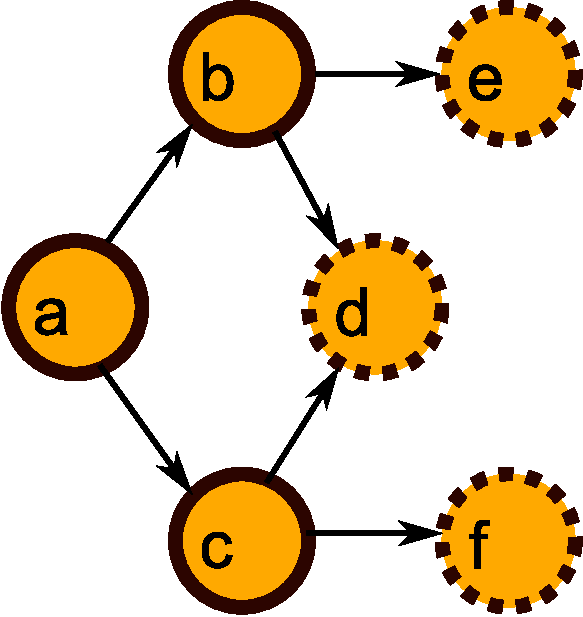
\includegraphics[width=4cm]{dependencies-one} 
    \end{center}
    \caption{\small Dependency diagram for a single forecast cycle in a
    simple example system. Tasks {\em a, b,} and {\em c} represent
    forecast models, and {\em d, e} and {\em f} are post processing or
    product generation tasks.} 
    \label{fig-dep-one} 
\end{figure} 

Figure \ref{fig-dep-one} shows a dependency diagram, which forms a {\em
Directed Acyclic Graph}, for a single forecast cycle of a simple example
system consisting of three forecast models ({\em a, b,} and {\em c}) and
three post processing or product generation tasks ({\em d, e} and {\em
f}).  Within a cycle each task may depend on one or more other
``upstream'' tasks, and may itself be depended on by one or more other
``downstream'' tasks.  A control system should therefore be capable of
managing, within a single forecast cycle, multiple parallel streams of
execution that branch when one task generates output for several
downstream tasks, and merge when one task takes input from several
upstream tasks. 

\begin{figure}
    \begin{center}
        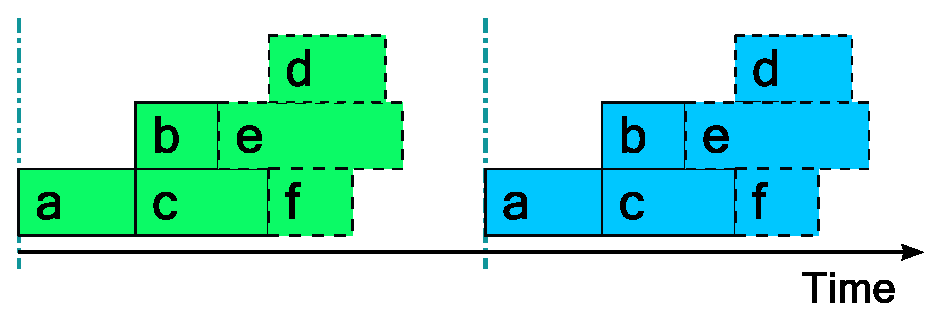
\includegraphics[width=8cm]{timeline-one}
    \end{center}
    \caption{\small Job schedule for two consecutive cycles of the
    example system during real time operation. The horizontal extent of
    a task bar represents execution time. Vertical sections through the
    graph intersect all tasks executing at that time, but the vertical
    ordering of tasks is not meaningful.}
    \label{fig-time-one}
\end{figure}

Figure \ref{fig-time-one} shows the job schedule for two consecutive
cycles of the example system in real time operation, given execution
times represented by the horizontal extent of the task bars. There is a
time gap between cycles as the system waits on new external driving
data. 
%and the schedule is optimal in the sense that every task begins
%executing as soon as its prerequisites are satisfied. 
All tasks here depend on upstream tasks {\em finishing} rather than on
any intermediate outputs, but this is just to make clearer diagrams.

\begin{figure} \begin{center}
    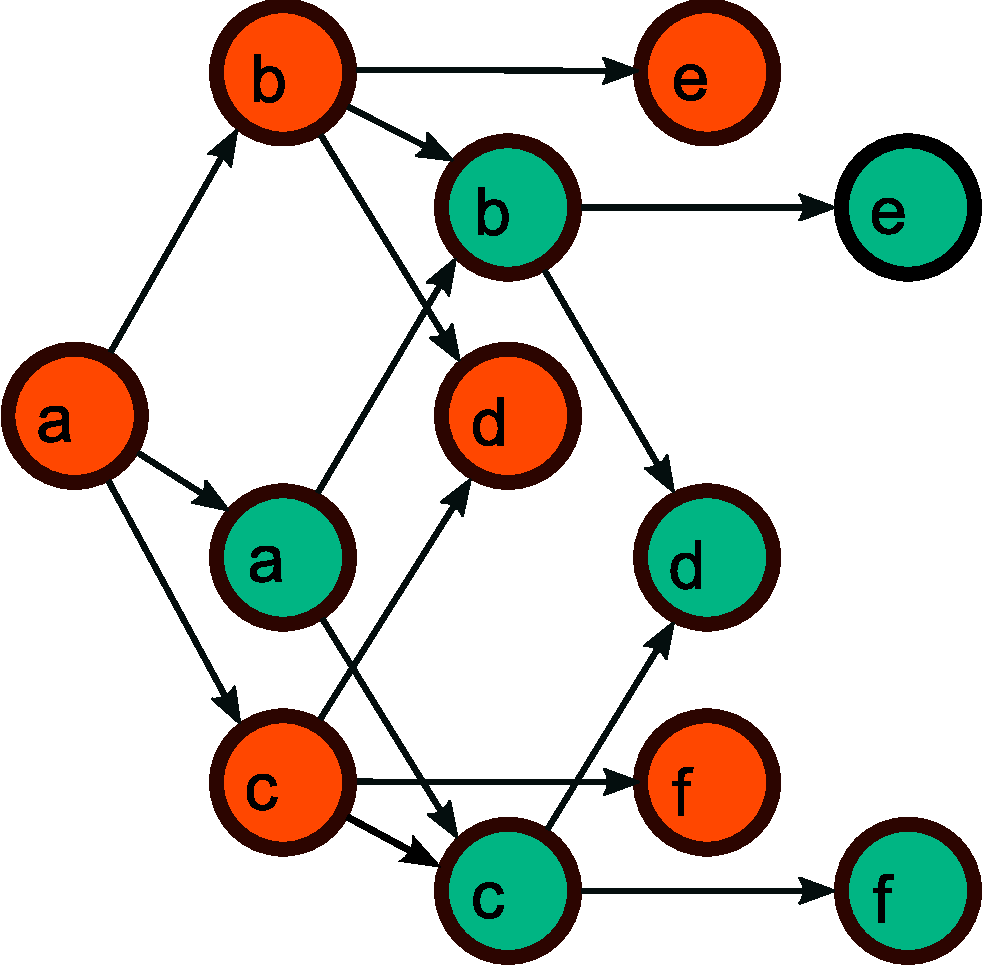
\includegraphics[width=6cm]{dependencies-two} \end{center}
    \caption{\small Complete dependency graph for the example
    system, assuming the least possible intercycle dependence: the
    forecast models ($a$, $b$, and $c$) depend on their own previous
    instances. The dashed arrows show connections to previous and
    subsequent forecast cycles.} 
    \label{fig-dep-two}
\end{figure}

Figure \ref{fig-dep-two} shows the complete dependency graph for the
example system, assuming the least possible intercycle dependence: each
forecast model ($a$, $b$, and $c$) depends on its own previous instance.

\begin{figure} 
    \begin{center} 
        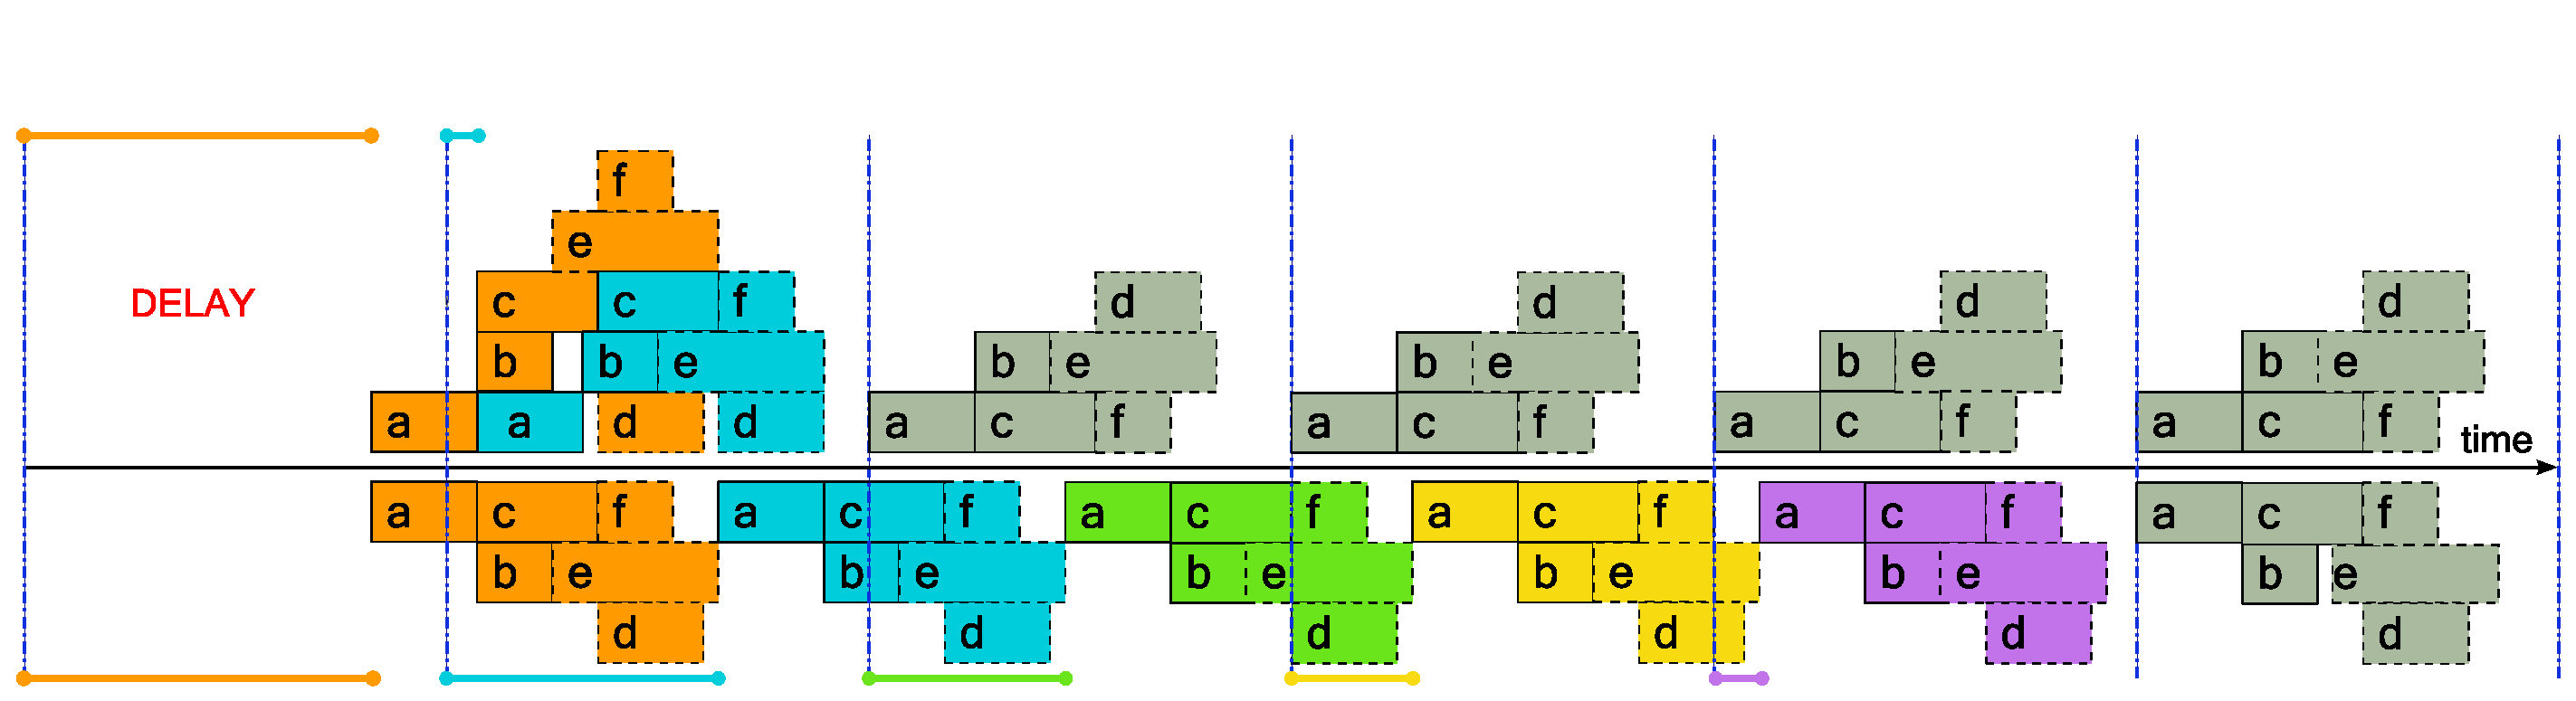
\includegraphics[width=12cm]{timeline-three}
    \end{center} 
    \caption{\small Job schedules for the example system after a delay
    of almost one whole forecast cycle, when intercycle dependencies are
    taken into account (above the time axis), and when they are not
    (below the time time axis). The colored lines indicate the time that
    each cycle is delayed, and normal ``caught up'' cycles
    are shaded gray.} 
    \label{fig-time-three}
\end{figure} 

Figure \ref{fig-time-three}, below the time axis, shows the effect of an
operational delay of almost one whole cycle on a sequentially cycling
system that has little downtime between cycles - it takes many cycles to
catch up. Above the time axis is the optimal schedule that is possible,
in principle, when intercycle dependencies are taken into account: the
second cycle after the delay is hardly affected, and subsequent cycles
all run on time.  Note that simply overlapping the single cycle
schedules of Figure \ref{fig-time-one} from the same start point would
have resulted in a dependency violation in task {\em c}.

\begin{figure} 
    \begin{center} 
        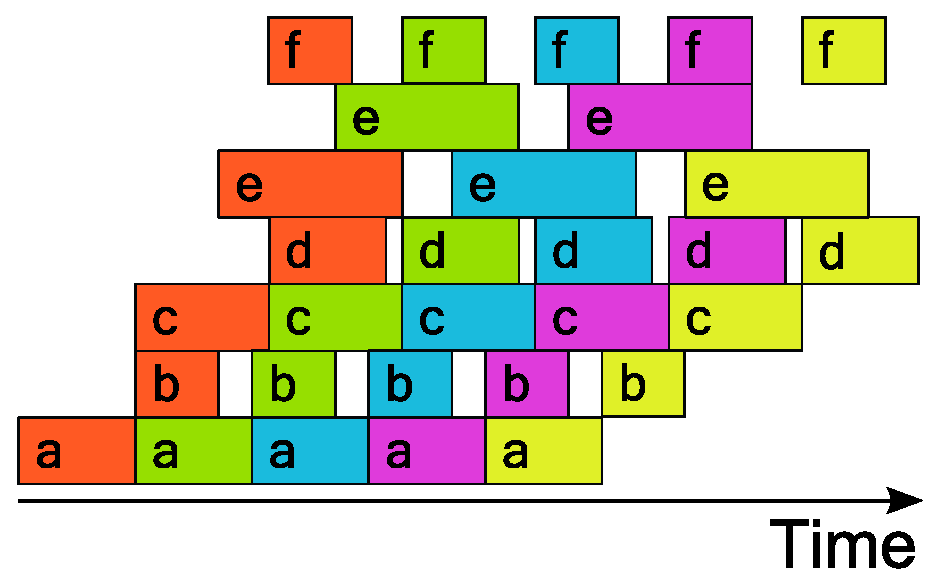
\includegraphics[width=8cm]{timeline-two}
    \end{center} 
    \caption{\small Job schedules for the example system in case study
    mode, or after a long delay, when the external driving data are
    available many cycles in advance. Above the time axis is the optimal
    schedule obtained when the system is constrained only by its true
    dependencies, as in Figure \ref{fig-dep-two}, and underneath it is
    the best that can be achieved when intercycle dependencies are
    ignored.} 
    \label{fig-time-two}
\end{figure} 

Similarly, Figure \ref{fig-time-two} shows job schedules for the example
system in case study mode, or when catching up after a very long delay,
when the external driving data are available many cycles in advance.
Task {\em a}, which as the most upstream forecast model is likely to be
a resource intensive atmosphere or ocean model, has no dependence on
cotemporal tasks and can therefore run continuously, regardless of how
much downstream processing is yet to be completed in its own cycle or in
any previous forecast cycle. In practice task {\em a} would depend on
cotemporal upstream tasks that wait on the external driving data, but
they would return immediately when the external data is available in
advance, so the result stands. Other tasks can cycle at regular short
intervals, the interval depending on [CHECK THIS] the task run length
relative to that of its longest cotemporal upstream dependency path. In
this case {\em c} can also run continuously, and consecutive instances
of {\em e}, which has no previous-instance dependence, can overlap.
Thus, even for this very simple example system, tasks from three or four
different cycles can run simultaneously, in principle, at any given
time. 

A new approach is required to achieve this because the hard coded
scheduling logic of the sequential cycling Finite State design above
already suffers from complexity-related problems, and extending it to
this more general system hardly seems feasible. The following section
describes the means by which cylon achieves continuous optimal
metascheduling. It smoothly transitions to a linear sequence of distinct
forecast cycles, as in Figure \ref{fig-time-one}, as the system catches
up to real time.  


\section{Cylon Implementation}

{\huge THIS SECTION IS VERY OUT OF DATE!}

\subsection{The Main Algorithm}

From the discussion above it is apparent that the additional complexity
due to explicitly handling intercycle dependencies is too difficult to
deal with in a Finite State Machine, and that the ``forecast cycle'' as
a global control system parameter has to be replaced with an independent
``forecast reference time'' for each task. This devolving of cycle
timing to the individual tasks suggests treating the system as a {\em
simulation} of autonomous proxy objects that represent the external
tasks and interact regardless of reference time to negotiate
dependencies at run time (i.e.\ by matching completed outputs against
prerequisites). If this can be made to work it provides extraordinary
power and flexibility because it treats all dependencies equally and it
makes any convoluted task scheduling logic entirely disappear: if task
proxy objects can interact indiscriminately then they don't need to know
{\em who} is supposed to satisfy their prerequisites and they can be
defined without reference to the other tasks in the system (except of
course that some other task(s) must exist that will satisfy their
prerequisites).  Existing tasks could be taken out of the system, or new
ones added, without changing the control system in any other way.
Further, by means of object polymorphism\footnote{Polymorphism is the
ability of one type to appear as and be used like another type. In OOP
languages with inheritance, this usually refers to the ability to treat
derived class objects as if they were members of a base class so that,
for instance, a group of mixed-type objects can all be treated as
members of a common base class while retaining their specialized derived
class behaviour.} the control system can be designed to automatically
handle any future task so long as it is derived from (inherits the
properties of) the original task base class.

The following simple description should be sufficient to enable the
reader to understand how the algorithm achieves optimal forecast
cycle-independent metascheduling. Everything else is arguably just
implementation, although some important aspects of that are not trivial
and will be discussed later.

\begin{itemize}
    \item The control system maintains a pool of autonomous {\em task
        proxy objects} that represent each real task. 
       
    \item The internal state of a task proxy object must reflect that
        of the real task it represents. This state information includes:

        \begin{itemize}

            \item task proxy object name.

            \item associated external (real) task.  

            \item owner of the real task, if necessary (who the task
                should run as).

            \item UTC {\em forecast reference time}, e.g. $2010012418$
        
            \item current execution status: {\em waiting}, {\em running}, 
                {\em finished}, or {\em failed}. 

            \item a list of prerequisites and whether or not they are
                satisfied yet, e.g.\ {\em file FOO is ready}. 

            \item a list of outputs completed so far, e.g.\ {\em file
                FOO is ready}.

        \end{itemize}
       
    \item A task proxy object can launch its associated external task
        when all of its prerequisites are satisfied.

    \item A task proxy object can interact with other task proxy
        objects (regardless of reference time; all dependencies are now
        equal) to determine if any of their completed outputs can
        satisfy any of its prerequisites.

    \item The control system gets the task pool to interact and
        negotiate dependencies whenever any new output is reported.
 
    \item A task proxy object must exist by the time it is needed to
        interact with other tasks, and must not cease to exist before
        it is no longer needed.

\end{itemize}

\subsubsection{Main Loop}

{\small
\noindent
\rule{5cm}{.2mm}
\begin{lstlisting}
while True:

   if task_base.state_changed:
       # PROCESS ALL TASKS whenever one has changed state
       # as a result of a remote task message coming in. 
       #---
       task_pool.process_tasks()
       task_pool.dump_state()
       if task_pool.all_finished():
           clean_shutdown( "ALL TASKS FINISHED" )

    # REMOTE METHOD HANDLING; handleRequests() returns 
    # after one or more remote method invocations are 
    # processed (these are not just task messages, hence 
    # the use of task_base.state_changed above).
    #---
    task_base.state_changed = False
    pyro_daemon.handleRequests( timeout = None )

# END MAIN LOOP
\end{lstlisting}
}


\label{sec-task-messaging}


\subsection{Task Proxy Object Life Cycle}

Task proxy creation and destruction must be managed so that, in a
continuously running system, they exist when needed, but do not exist
for too long before they are needed, and cease to exist soon after they
are no longer needed.

\subsubsection{Task Creation}

A task proxy object needs to exist, at the latest, by the time that all
of its prerequisites have been satisfied.  The earliest a task can run
is governed chiefly by whether it depends on its previous
instance (in which case it can potentially run as soon as its previous
instance has finished\footnote{Or when it has generated its background
state for the next instance, at least.}) or not (in which case it can
potentially run in parallel with its previous instance). This
information is specific to the task type so the best place to hold it is
in the task proxy class definitions. 

New tasks are therefore created after their previous instance {\em
abdicates}; for forecast models this happens when the previous instance
finishes\footnote{But see previous footnote}; and otherwise as soon as
the previous instance starts running. This ensures that a task cannot
run before its previous instance without use of explicit intercycle
prerequisites that would require special treatment at startup (when
there is no previous cycle). Tasks are not deleted immediately on
abdication (see below).

\subsubsection{Removing Spent Tasks} 

A task is spent if it finished {\em and} no longer needed to satisfy the
prequisites of any other task. Most tasks are only needed by other
cotemporal downstream tasks; these can be removed when they are finished
{\em and} older than the oldest non-finished task. For rare cases that
are needed by tasks in later reference times (e.g.\ nzlam post
processing: multiple hourly topnet tasks need the same most recent
previously finished 06 or 18Z nzlam post processing task), each
non-finished task reports its {\em cutoff reference time} which is the
oldest reference time that may contain tasks still needed to satisfy its
own prerequisites (if it is waiting) or those of its immediate
post-abdication successor (if it is running already), then the task
manager can then kill any finished tasks that are also older than the
oldest task cutoff time.

\subsubsection{Removing Lame Tasks} 

Tasks that will never run (because their prerequisites cannot be
satisfied by any other task in the system) are removed from the {\em
oldest batch} of tasks.  If not removed they would prevent the spent
task deletion algorithm from working properly. Lame tasks can only be
detected in the oldest task batch; in younger batches some tasks may yet
appear as their predecessors abdicate.

Lame tasks are abdicated rather than just deleted, because their
descendents will not necessarily be lame: e.g.\ if the system is started
at 12Z with topnet turned on, all topnet tasks from 12Z through 17Z will
be valid but lame, because they will want to take input from a
non-existent nzlam\_post from 06Z prior to startup. However, the
presence of lame tasks may indicate user error: e.g.\ if you forget
to turn on task type $foo$ that supplies input to task type $bar$,
any instance of $bar$ will be lame.

\subsection{Constraining The System}

No task is allowed to get more than 48 hours (user configurable) ahead
of the slowest task in the system (with respect to reference time).


\subsection{Coupling Task Proxies to Tasks} 

Our task proxy objects must keep track of progress in their external
counterparts. Most task prerequisites are just files generated by other
tasks, so it is tempting to have the controller use the appearance of
expected new output files as a proxy for task progress. But we have to
be sure that a newly detected file is complete, not just that it exists,
and it is difficult to do this in an OS-independent way (using {\em
inotify} on Linux, for example.). 
%On Linux one could insist that every completed output file is
%immediately renamed by the generating task, and have the controller use
%{\em inotify} to watch for the sudden appearance of the new file
%(because file rename operations are atomic when the source and target
%are on the same file system) [REF: Simon, if he wants]. But this is not
%platform independent, and most forecast systems run on heterogeneous
%distributed hardware. 
More importantly though, prerequisites are not necessarily single files:
a task could conceivably depend on completion of a large set of files, a
database update, or a data transfer by remote procedure call, for
instance. Consequently we chose to use a high level messaging system for
communication between external tasks and the control system. This is
platform independent and allows tasks to be triggered off any
conceivable condition. For example, rather than detecting the existence
of the file {\em FOO}, the controller would receive a message saying
{\em file FOO is ready}, or similar, from the task that has
just generated the file.  There is no need for the control system itself
does to verify that the message is true (i.e. that file {\em FOO}
really does exist) because any downstream task that
depends on file {\em FOO} must necessarily do that itself, and error 
conditions can be reported back to the controller, and possibly to a
separate monitoring system as well, at that point.

The Python Remote Object Protocal (Pyro) allows external programs to
communicate directly, across the network, with specific objects inside
the running controller. This means that tasks can communicate directly
with their own proxy objects, obviating the need for any any internal
message brokering mechanism in the control system.    

Each task must express its prerequisites (i.e.\ its dependence on
upstream tasks) as a text string, for example ``file X is ready'', or
``task X has completed'', or ``task X has completed writing all Y
files'', and must send messages of the same kind back to the controller
to indicate when it has reached an important waypoint or completed
generated any important outputs.  


\subsection{Task Definition}
blah.

\subsection{Pyro}
blah.

\subsection{Pure Simulation Mode}

The dynamic metascheduling algorithm is essentially a simulation of an
interacting task set in which the state of each task proxy object is
coupled to that of the real task it represents. In addition, task proxy
state changes occur in response to {\em messages} rather than, say,
actual detection of newly generated input files.  This suggests
a {\em dummy mode} in which each configured external task is replaced by
an instance of an external dummy program that masquerades as the real
task by reporting completion of each of its outputs in turn (task output
lists can be exposed to other programs, namely to the dummy task
program, through Pyro RPC calls). As far as the control system is
concerned this is indistinguishable from real operation, except that
external dummy tasks are less likely to be delayed by resource
contention, and the dummy mode can be run according to an accelerated
clock, rather than real time, for quick testing.  Dummy tasks therefore
complete in approximately the same dummy clock time as the real tasks do
in real time. An initial dummy clock offset relative to the initial
reference time can also be specified, which allows simulation of the
transition between catch up and real time operation, and vice versa. Log
messages are stamped with dummy clock time instead of real time.

The same script is used for all external dummy tasks but it has special
behaviour in certain cases: the dummy downloader ``waits for incoming
files'' until 3:15 past its reference time, and the dummy topnet ``waits
for stream flow data'' until 0:15 past its reference time.

The dummy clock can be bumped forward a number of hours by remote
control, while the system is running. This affects the postrequisite
timing of running tasks correctly, but if it causes a running task to
finish immediately the next task in line will still start from the
beginning no matter how big the bump.



%some tasks, such as those that wait on external input data, and tide
%models, may have no upstream dependencies at all.

%This could be done by checking for the existence of required inputs
%directly, or by monitoring the state of the other tasks that are known
%to provide the inputs in each case (are they finished yet?).  

%The control program thus remains simple and generic, regardless of the
%number of tasks or the complexity of their interdependencies; it simply
%manages a set of tasks that are all individually configured as if they
%were to run in isolation.\footnote{The system manager does of course
%have to ensure that the configured task pool is self consistent, i.e.\
%that each task's prerequisites will be satisfied by some other task(s)
%in the system.}
%The total absence of explicit scheduling logic makes this method
%extremely flexible and extensible.\footnote{To extend the system, one
%simply derives a new class definition that lists the new task's
%prerequisites and outputs. The new task will automatically run at the
%right time, i.e.\ when its prerequisites have been satisfied by some
%other task(s) in the system.}


\subsection{Applicability}

The object oriented dynamic metascheduling concept is quite general and
could in principle be implemented for any set of interdependent tasks.
cylon, however, is specialized toward cycling forecast systems in that
each task must have an associated {\em forecast reference time} that is
part of a predetermined series for a given task type and is not
necessarily related to the real time at which the task actually runs.  

\subsection{Environment}

EcoConnect operates in a well defined environment so that each real task
knows what its input files look like for a given reference time
(through filenaming conventions) and where to get them from (e.g.\ from
their own input directories, or upstream output directories).
Consequently the control system does not need to know the location of
important input/output files, just (via messaging) that they exist. In a
less structured environment additional tasks could easily be added to
to move files around as needed. 

\subsection{Startup and Initialization}

An initial reference time and list of task object names are read in from
the config file, then each task object is created at the initial
reference time {\em or} at the first subsequent reference time that is
valid for the task type. Optionally, we can tell the controller to
reload the current state dump file (which may have been edited); this
will override the configured start time and task list. After startup,
new tasks are created only by {\em abdication} (below).

An initial run through the {\em task processing} code, by virtue of the
fact that the main loop starts with task processing, causes tasks with
no prerequisites (e.g.\ {\em downloader}) to enter the {\em running}
state and launch their external tasks immediately. Otherwise ({\em or}
if there are no tasks that lack prerequisites) nothing will happen.


\subsection{Task Interaction} 

Each task keeps track of which of its postrequisites are completed, and
asks the other tasks if they can satisfy any of its prerequisites. 

{\small
\noindent
\rule{5cm}{.2mm}
\begin{lstlisting}
class task_pool( Pyro.core.ObjBase ):
    # ...
    def interact( self ):
        # get each task to ask all the others if 
        # they can satisfy its prerequisites
        #--
        for task in self.tasks:
            task.get_satisfaction( self.tasks )
    # ...
\end{lstlisting}
}

\subsection{Running Tasks}

Each task object can launch its associated external task, and enter the
{\em running} state if its prerequisites are all satisfied, any existing
older tasks of the same type are already {\em finished}, and fewer than
{\em MAX\_ RUNAHEAD} finished tasks of the same type still exist (this
stops tasks with no prerequisites from running ahead indefinitely).

\subsection{Pyro Remote Method Calls}

The Pyro request handling loop executes remote method calls coming in
from external tasks, and returns after at least one call was handled.
Pyro must be run in non-default single-threaded mode (see Appendix
\ref{pyro-appendix}).

\subsection{Dumping State} 

The current state (waiting, running, or finished) of each task is
written out to the {\em state dump file}.  This provides a running
snapshot of the system as it runs, and just prior to shutdown or
failure. The controller can optionally start up by loading the state
dump (which can be edited first). Any 'running' tasks are reloaded in
the 'waiting' state.

\appendix

\section{Essential OOP Concepts}

The simplicity of the dynamic scheduling implementation in {\em cylon}
is critically dependent on the {\em polymorphic} nature of the {\em task
objects} in the program.  This section contains a minimal introduction
to these Object Oriented Programming concepts.  Refer to any OOP
reference for more detail.

\subsection{Classes and Objects}

A {\em class} is essentially a generalisation of {\em data type} to
include {\em behaviour} (i.e.\ functions or {\em methods}) as well as
state.  {\em Objects} are more or less self contained {\em instances} of
a class. For example, a $shape$ class could define a $position$ data
member that describes the location of each shape object, a $move()$
method that causes a shape object to alter its position, and a $draw()$
method that causes it to display itself in the right place on screen.

\subsection{Inheritance}

A {\em derived class} or {\em subclass} inherits the properties (methods
and data members) of a {\em base class}. It can also {\em override}
specific base class properties, or add new properties that aren't
present in the base class. Calling a particular method on an object
invokes the object's own class method if one is defined, otherwise the
immediate base class is searched, and so on down to the root of the
inheritance graph. 

For example, we could derive a $circle$ class from $shape$, adding a
`radius' data member and overriding the $draw()$ to get circle objects
to display themselves as actual circles.  Because we didn't override the
$move()$ method, calling $circle.move()$ would invoke the base class
method, $shape.move()$. 


\subsection{Polymorphism}

Polymorphism is the ability of one type to appear as and be used like
another type.  In OOP languages with inheritance, this usually refers to
the ability to treat derived/sub-class objects as if they were members
of a base class.  In particular, a group of mixed-type objects can all
be treated as members of a common base class. For example, we could
construct a list of $shape$ objects from $circles$, $triangles$, and
$squares$; calling $[list member].draw()$ will invoke the right derived
class $draw()$. This is a very powerful mechanism because {\em it allows
unmodified old code to call new code}: if we later derive an entirely
new kind of shape ($hexagon$, say) with it's own unique behaviour, the
existing program, without modification, will process the new objects in
the proper hexagon-specific way.


\section{Threading in Pyro} \label{pyro-appendix}

With Pyro in {\em single threaded mode}, \verb#handleRequests()# returns
after {\em either} a timeout has occurred {\em or} at least one request
(i.e.\ remote method call) was handled. With \verb#timeout = None# this
allows us to process tasks {\em only} after remote method invocations
come in.  Further, we can detect the remote calls that actually change
task states, and thereby drop into the task processing code only when
necessary, which minimizes non-useful output from the task processing
loop (e.g.\ in dummy mode there are a lot of remote calls on the dummy
clock object, which does not alter tasks at all). 

In {\em multithreaded mode}, \verb#handleRequests()# returns immediately
after creating a new request handling thread for a single remote object
and thereafter remote method calls on that object come in asynchronously
in the dedicated thread. This is not good for the dynamic scheduling
algorithm because tasks are only set running in the task processing
block which can be delayed while \verb#handleRequests()# blocks waiting
for a new connection to be established even as messages that warrent
task processing are coming in on existing connections. The only way
around this is to do task processing on \verb#handleRequests()# timeouts
which results in a lot of unnecessary task processing when nothing
important is happening.


\subsection{Interfacing Tasks To cylon}
blah.

\subsection{Utility Programs}
blah.

\subsubsection{Configure System}
blah.

\subsubsection{Remote Control}
blah.

\subsubsection{System Monitors}
blah.

\subsection{Logging}
blah.

\section{Miscellaneous Notes}

\subsection{Product Generation}

Note that ``correct scheduling'' is not necessarily equivalent to
``orderly generation of products by reference time'' (the upstream 
forecast model can run continuously regardless of any downstream
processing that depends on it).

\subsection{Catching Up}

The state of ``catching up'' is a property of the individual tasks, not
the whole system. Where this matters, it can be detected by the relevant
external task. E.g.\ if the external topnet(T) task starts up at real
time t greater than the stream flow data time for T (i.e.\ $T+15$ min),
i.e.\ the required stream flow data is already available, then we're
still in catch up. If, on the other hand, the topnet task finds that it
has to wait for its stream flow data time to arrive, then we're caught
up to real time.  This matters because topnet is allowed to run ahead by
a different amount of time depending on whether we're in catch up mode or
not.

\subsection{Controlling Task Execution}

\begin{itemize}
 \item  prerequisites
 \item artificial prerequisites (e.g.\ make nztide depend on nzlam)
 \item delayed instantiation (a task can't run if it doesn't exist yet).
 \item other contraints based on, for example, the number of previous
 instances that still exist in the system, or how far ahead of the 
 slowest/oldest task we can get.
\end{itemize}

\subsection{fuzzy prequisites}

{\em Exact prerequisites} (most tasks): times are specified exactly,
relative to the task's own reference time.  E.g.\ {\em file foo\_{T}.nc
ready} where T is the task's reference time.

{\em Fuzzy prerequisites} (topnet): a time boundary is specified
relative to the task's own reference time; any task with a reference
time greater than or equal to the boundary time can satisify the
prerequisite.

\end{document}
